\documentclass[../jarvis.tex]{subfiles}
\usepackage{hyperref}
\newscrambledenv{hint}
\graphicspath{{\subfix{../images/}}}

\begin{document}
As it turns out, there's more to algebra than pure uninspiring symbol pushing. In this chapter we look at some structures and concepts in elementary algebra.

\begin{figure}[H]
    \centering
    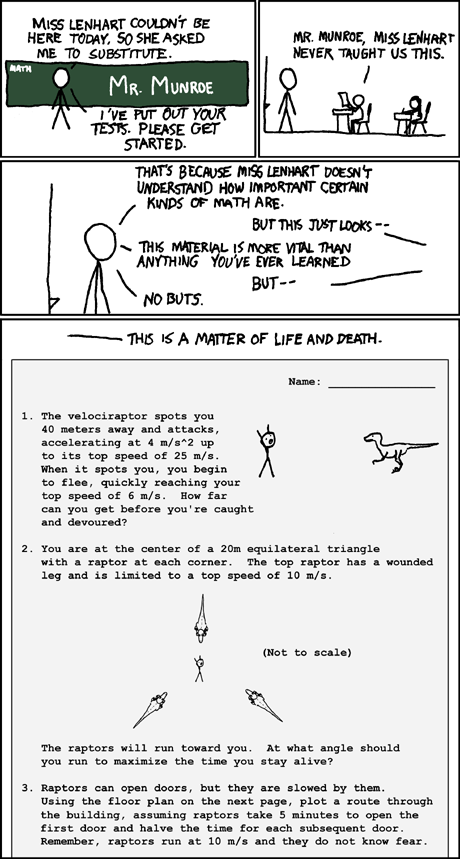
\includegraphics[scale=0.55]{xkcd_substitute.png}
    \caption{Comic from https://xkcd.wtf/135/}
\end{figure}

\section{Many Manipulations}
\subsection{Factorising and Re-expressing}
These techniques are most useful when we are faced with some funny-looking problems that solve themselves after some smart rearranging and rewriting.

\begin{example}[2013 SMO(J) P15]
    If $a=1.69$, $b=1.73$ and $c=0.48$, find the value of
    $$\frac{1}{a^2-ac-ab+bc}+\frac{2}{b^2-ab-bc+ac}+\frac{1}{c^2-ac-bc+ab}.$$
\end{example}
Of course, a good calculator can do this in seconds (although typing it in may take longer...), but what if you had to do this by hand? Substituting may not be smart...

However, we note that each of the denominators are suspiciously factorisable. For example,
$$a^2-ac-ab+bc=a(a-c)-b(a-c)=(a-b)(a-c).$$

\begin{proof}
    Hence,
\begin{align*}
    & \frac{1}{a^2-ac-ab+bc}+\frac{1}{b^2-ab-bc+ac}+\frac{1}{c^2-ac-bc+ab}\\
    &=\frac{1}{(a-b)(a-c)}+\frac{2}{(b-c)(b-a)}+\frac{1}{(c-b)(c-a)} \\
    &=\frac{(b-c)-2(a-c)+(a-b)}{(a-b)(a-c)(b-c)} \\
    &=-\frac{1}{(a-b)(b-c)} = -\frac{1}{(-0.04)(1.25)} = \boxed{20}
\end{align*}
\end{proof}

\begin{example}[2013 SMO(J) P20]
    Let $a,b,c$ be real numbers such that $\frac{ab}{a+b}=\frac{1}{3}$, $\frac{bc}{b+c}=\frac{1}{4}$ and $\frac{ca}{c+a}=\frac{1}{5}$. Find the value of $\frac{24abc}{ab+bc+ca}$.
\end{example}
Of course, taking the given equations as-is gives us no room to work with. We do want to split up the fractions somehow though, and the denominators seem easy for us to work with: lets bring them to the numerator instead.

Indeed, we observe that $\frac{a+b}{ab}=\frac{1}{a}+\frac{1}{b}$.
\begin{proof}
    Taking reciprocals, we have
    $$
    \begin{cases*}
        \frac{1}{a}+\frac{1}{b} &= 3\\
        \frac{1}{b}+\frac{1}{c} &= 4\\
        \frac{1}{c}+\frac{1}{a} &= 5 \\
    \end{cases*}
    \implies \frac{1}{a}+\frac{1}{b}+\frac{1}{c}=6.$$
    
    Let $S$ denote our desired expression. With a similar idea, 
    $$\frac{1}{S}=\frac{1}{24}\left(\frac{1}{a}+\frac{1}{b}+\frac{1}{c}\right)=\frac{1}{4} \implies S=\boxed{6}.$$
\end{proof}

\begin{example}[2013 SMO(J) P32]
    If $a$ and $b$ are positive integers such that $a^2+2ab-3b^2-41=0$, find $a^2+b^2$.
\end{example}
The constant "$41$" seems irrelevant to the equation at this point, except that it's a prime number (this may be important!). For now, let us write the equation as $a^2+2ab-3b^2=41$.

\begin{proof}
    Notice that the coefficients of the LHS sum to $(1+2-3=)0$(!), so this tells us that we should factorise:
$$a^2+2ab-3b^2=a^2-ab+3ab-3b^2=a(a-b)+3b(a-b)=(a+3b)(a-b)=41.$$

Now, it becomes apparent why $41$ was chosen: because it is a prime number, and $a,b$ are integers, $a+3b$ and $a-b$ are each either $1$ or $41$. Moreover, $a+3b \geq a-b$ so we have
$$
\begin{cases}
    a+3b&=41 \\
    a-b&=1
\end{cases} \implies a=11, b=10.
$$
Thus, $a^2+b^2=11^2+10^2=\boxed{221}$.
\end{proof}


\begin{example}[2017 SMO(J) P20]
    Let $a$, $b$ and $c$ be positive integers such that
    $$a^2+bc=257\quad\text{and}\quad ab+bc=101.$$

    Find the value of $a$, $b$ and $c$.
\end{example}
\begin{proof}
    Armed with the idea from the previous problem, we see again that $101$ is a prime number, so $b(a+c)=101$. Moreover, $b+c\geq a$ so that $b=1$ and $a+c=101$. Thus, $$a^2+bc=a^2+c=a^2+(101-a)=257 \implies a(a-1)=156.$$

    With some guess and check (since $a$ is a positive integer), $a=13$, $b=1$ and $c=88$.
\end{proof}


\begin{example}[2016 SMO(J) P24]
    If $\frac{a}{2b}=\frac{2b}{3c}=\frac{3c}{8a}$, find the value of $\frac{ac+cb}{cb-ba}.$
\end{example}
The given condition tells us that $a$, $b$ and $c$ are all connected, so we should express $a$ and $b$ in terms of $c$.

\begin{proof}
    Let $\frac{a}{2b}=\frac{2b}{3c}=\frac{3c}{8a}=k$ for some real $k$. We have
$$ 
\begin{cases}
    a=2kb \\
    2b=3kc \\
    3c=8ka
\end{cases}
\implies
\begin{cases}
    a=3k^2c \\
    2b=8k^2a \\
\end{cases}
\implies
\begin{cases}
    a=24k^5c \\
    b=12k^4c    
\end{cases} 
.$$
By the given condition, we have $\frac{2b}{3c}=\frac{24k^4c}{3c}=8k^4=k \implies 8k^3=1 \implies k=\frac{1}{2}$, $k^5=\frac{1}{32}$

Hence,
\begin{align*}
    \frac{ac+cb}{cb-ba}
    &= \frac{24k^5c^2+12k^4c^2}{12k^4c^2-288k^9c^2} \\
    &= \frac{2k+1}{1-24k^5} \\
    &= \frac{2\cdot\frac{1}{2}+1}{1-24\cdot\frac{1}{32}} = \boxed{8}
\end{align*}
\end{proof}

\subsection{Homogenisation}
For our first concept of the handout, we introduce the trick of counting degrees, or \textit{homogenisation}. We only illustrate as such with a simple problem, and further applications of this idea will follow in a later.

\begin{proposition}[Counting degrees]
    We say that an expression or equation is \textit{homogenous} (or homogenised) if there is no loose constant terms remaining. For example, $x^3+2022x^2y+2021$ is non-homogenous because of the constant $2021$, while $x^3+2022xy^3+xy$ is homogenous because there is no loose constant. 

    We \textit{want} to work with homogenous expressions because degrees cancel nicely, and expressions are usually neat. 
\end{proposition}
\begin{example}
    If $x$ and $y$ are real numbers such that $x+y=2$ and that
    $$\frac{(1-x)^2}{x}+\frac{(1-y)^2}{y}=-4,$$
    find the value of $xy$.
\end{example}

Consider the term $\frac{(1-x)^2}{x}$. The numerator is a quadratic (degree $2$) while the denominator is linear (degree $1$), so we say that this term is of degree $1$. The term $\frac{(1-y)^2}{y}$ is also similarly of degree $1$, and so the LHS is of degree $1$. 

On the other hand, the RHS is a constant (degree $0$), which makes the equation \textit{non-homogenous}. Fortunately, we are given that $x+y=2$. 

\begin{proof}
    We begin by writing
$$\frac{(1-x)^2}{x}+\frac{(1-y)^2}{y}=-2(x+y).$$ Now, our equation is homogenous, and as we shall see, this equation now resolves itself very cleanly. Clearing denominators (since $x,y \neq 0$), we have
\begin{align*}
    \frac{(1-x)^2}{x}+\frac{(1-y)^2}{y}=-2(x+y) &\implies x(1-y)^2+y(1-x)^2=-2xy(x+y) \\
    &\implies (xy^2-2xy+x)+(x^2y-2xy+y)=-2x^2y-2xy^2 \\
    &\implies 3x^2y+3xy^2-4xy+(x+y)=0 \\
    &\implies 3xy(x+y)-4xy+(x+y)=0 \\
    &\implies 2xy+2=0 \implies xy=\boxed{-1}
\end{align*}
\end{proof}

\subsection{Substitutions and Identities}
Sometimes scary expressions are just expanded versions of simpler expressions! A smart substitution will help simplify things nicely. Certainly, knowing some basic identities will help reduce the problem. Here, we list the necessary few.

\begin{proposition}[Basic Identities]
    These identities can also be found in school textbooks, and familiarity is assumed.
    \begin{enumerate}
        \item $a^2-b^2=(a-b)(a+b)$
        \item $a^2\pm 2ab+b^2=(a\pm b)^2$
        \item $a^3\pm b^3=(a\pm b)(a^2\mp ab+b^2)$
        \item $a^3+3a^2b+3ab^2+b^3=(a+b)^3$
        \item $a^3-3a^2b+3ab^2-b^3=(a-b)^3$
    \end{enumerate}
\end{proposition}

To start off, we showcase an application of a nifty substitution, without which, the problem may be untractable to the unsuspecting student.
\begin{example}[2013 SMO(J) P11]
    Find the value of $\sqrt{9999^2+19999}.$
\end{example}
Certainly, we are not expected to multiply out and then take the square root of this monstrous expression! However, we do note that the choice of $9999$ is completely arbitrary, so it may be wise to make a substitution for $9999$ and express $19999$ in terms of $a$.

\begin{proof}
    Let $a=9999$, then $19999=2\cdot 9999+1=2a+1$. Aha! We now know
\begin{align*}
    \sqrt{9999^2+19999}&=\sqrt{a^2+(2a+1)} \\
    &=\sqrt{(a+1)^2}=a+1 \\
    &=\boxed{10000}.
\end{align*}
How nice is that!
\end{proof}

\begin{example}[2014 SMO(J) P16]
    Let $m$ and $n$ be positive real numbers satisfying the equation
    $$m+4\sqrt{mn}-2\sqrt{m}-4\sqrt{n}+4n=3.$$
    Find the value of $$\frac{\sqrt{m}+2\sqrt{n}+2014}{4-\sqrt{m}-2\sqrt{n}}.$$
\end{example}
The required value is just as grizzly as the given equation. To start, we should be somewhat suspicious of the term $4\sqrt{mn}$: this is a term of degree $1$, since $\sqrt{m}$ and $\sqrt{n}$ both have degree $\frac{1}{2}$. Yet, it's mixed in an expression containing terms of degree $\frac{1}{2}$ like $2\sqrt{m}$ and $4\sqrt{n}$, as well as degree $1$ terms like $m$ and $4n$.

This strongly suggests the substitutions $x=\sqrt{m}, y=\sqrt{n}$, so we want the value of 
$$\frac{\sqrt{m}+2\sqrt{n}+2014}{4-\sqrt{m}-2\sqrt{n}}=\frac{x+2y+2014}{4-(x+2y)}.$$

The given equation gives $$x^2+4xy-2x-4y+4y^2=3. \implies (x+2y)^2-2(x+2y)=3 \implies (x+2y)(x+2y-2)=3.$$ Setting $z=x+2y$, $z(z-2)=3 \implies z^2-2z-3=0 \implies z=3$ only since $z=x+2y>0$. 

Hence, the required value is \boxed{4}.

\begin{example}[2015 SMO(J) P21]
    Find the value of $$\sqrt{(98\cdot 100+2)(100\cdot 102+2)+(100\cdot 2)^2}.$$
\end{example}
Once again, this is a monstrous expression, but fortunately the individual parts in the expression are broken down slightly for us. For now, let us focus on the term $98\cdot 100+2$. 

It may be tempting to simply substitute $a=98$ (or $a=100$), but the expression $a(a+2)+2=a^2+2a+2$ is cumbersome to work with. Perhaps we should compromise and let $a=99$ instead!

Then, $98\cdot 100+2= (a-1)(a+1)+2=a^2+1=99^2+1$, and similarly, $100\cdot 102+2 = 101^2+1$. The desired expression is now
$\sqrt{(99^2+1)(101^2+1)+(100\cdot 2)^2}$, and it is apparent why $100\cdot 2$ was written instead of $200$. Letting $b=100$, we have
\begin{align*}
    \sqrt{(99^2+1)(101^2+1)+(100\cdot 2)^2}&=\sqrt{((b-1)^2+1)((b+1)^2+1)+4b^2}\\
    &=\sqrt{(b^2-2b+2)(b^2+2b+2)+4b^2} \\
    &=\sqrt{((b^2+2)-2b)((b^2+2)+2b)+4b^2} \\
    &=\sqrt{(b^2+2)^2-(2b)^2+4b^2} \\
    &= b^2+2=\boxed{10002}
\end{align*}

\begin{example}[2018 AMC10 A/10]
    Suppose that real number $x$ satisfies $$\sqrt{49-x^2}-\sqrt{25-x^2}=3.$$
    Find the value of $\sqrt{49-x^2}+\sqrt{25-x^2}$.
\end{example}
The given equation is an equation in terms of $x^2$, so it would be instinctive to substitute $y=x^2$ and then squaring both sides and rearranging:
\begin{align*}
    \sqrt{49-y}-\sqrt{25-y}=3 &\implies 74-2y-2\sqrt{(49-y)(25-y)}=9 \\
    &\implies 2\sqrt{(49-y)(25-y)}=65-2y\\
    &\implies 4(49-y)(25-y)=(65-2y)^2 \\
    &\implies 4(y^2-74y+1225)=4y^2-260y+4225 \\
    &\implies -36y+675=0 \implies y=\frac{75}{4},
\end{align*}
whence the required value is 
$$\sqrt{49-x^2}+\sqrt{25-x^2}=\sqrt{49-y}+\sqrt{25-y}=\sqrt{\frac{121}{4}}+\sqrt{\frac{25}{4}}=\boxed{8}.$$

This method feels slightly disingenous though, why would the problem seek such a specific quantity? On a closer look, we notice that the given expression and the required expression are very similar. In particular, they differ only in their signs!

If we let $a=\sqrt{49-x^2}$ and $b=\sqrt{25-x^2}$, then $a-b=3$ and we seek the value of $a+b$.

This reminds us of the \textit{difference of squares} identity, and we finish the problem succinctly:
\begin{proof}
    $$(a-b)(a+b)=a^2-b^2=(49-x^2)-(25-x^2)=24.$$
On the other hand, 
$$3(a+b)=24 \implies \sqrt{49-x^2}+\sqrt{25-x^2}=a+b=\frac{24}{3}=\boxed{8}.$$
\end{proof} 

For our ending problem, we showcase the idea of \textit{rationalisation} for cube roots. Indeed, at the heart of rationalising surds, we rely on the difference of squares. As it turns out, this also works for cube roots! 
\begin{example}[2013 AIME II/5]
    Find the real root of the equation $8x^3-3x^2-3x-1=0$ in the form 
    $$x=\frac{\cbrt{a}+\cbrt{b}+1}{c},$$
    where $a,b,c$ are positive integers.
\end{example}
Firstly, the coefficients $3, 3, 1$ seem vaguely familiar. In fact, $(x+1)^3=x^3+3x^2+3x+1$. Thus, we write
$$8x^3-3x^2-3x-1=9x^3-(x^3+3x^2+3x+1)=9x^3-(x+1)^3,$$
whence $9x^3=(x+1)^3$.

Solving for $x$, we have $$x=\frac{1}{\cbrt{9}-1}.$$ We make the substitution $a=\cbrt{9}$, and so $a^3=9$. The cube root suggests that the difference of cubes formula may be useful. Indeed, $$(a-1)(a^2+a+1)=a^3-1,$$ and so
\begin{align*}
    x&=\frac{1}{\cbrt{9}-1}=\frac{1}{a-1} \\
    &=\frac{1}{a-1}\cdot \frac{a^2+a+1}{a^2+a+1}=\frac{a^2+a+1}{a^3-1} \\
    &=\frac{\cbrt{81}+\cbrt{9}+1}{8}.
\end{align*}

\subsection{Exercises}
\problem[2015 SMO(J) P9]Find the value of $\left(4\sqrt{4+2\sqrt{3}}-\sqrt{49+8\sqrt{3}}\right)^2.$
\begin{hints}
    \begin{hint}
        Simplify the square roots.
    \end{hint}
\end{hints}
\problem[2014 SMO(J) P13]Let $A$ be the solution of the equation
$$\frac{x-7}{x-8}-\frac{x-8}{x-9}=\frac{x-10}{x-11}-\frac{x-11}{x-12}.$$
\begin{hints}
    \begin{hint}
        Each numerator isn't \textit{that} different from it's denominator.
    \end{hint}
\end{hints}
\problem[2016 SMO(J) P11]If the sum and product of two positive real numbers are both equal to $13$, find the sum of the squares of these two numbers.
\problem[2022 SMO(J) P22]If we have $$\frac{\sqrt{15}+\sqrt{35}+\sqrt{21}+5}{\sqrt{3}+2\sqrt{5}+\sqrt{7}}=\frac{a\sqrt{7}+b\sqrt{5}+c\sqrt{3}}{2}$$ for some integers $a,b,c$, find their values.
\begin{hints}
    \begin{hint}
        Note that $\sqrt{3}+2\sqrt{5}+\sqrt{7}=(3+\sqrt{5})+(\sqrt{5}+\sqrt{7})$
    \end{hint}
    \begin{hint}
        Use one of the first few examples for an inspiration.
    \end{hint}
\end{hints}
\problem[2014 SMO(J) P23]Let $a,b,c$ be non-zero reals satisfying $a+2b+3c=2014$ and $2a+3b+2c=2014$, find the value of 
$$\frac{a^2+b^2+c^2}{ab+bc+ca}.$$
\problem[2014 SMO(J) P26]Let $x$ be such that $\left(x+\frac{1}{x}\right)^2=3$. Evaluate $x^3+\frac{1}{x^3}.$
\problem[2014/15 SDML 2A/P5]Let $a,b,c,d,e$ be five consecutive positive integers such that $a<b<c<d<e$. If $b+c+d$ is a perfect cube and $a+b+c+d+e$ is a perfect square, find the smallest possible value of $e$.
\problem[2008 SMO(J) P23]Evaluate 
$$\frac{(2020^2-20100)(20100^2-100^2)(2000^2+20100)}{2010^6-10^6}.$$
\problem[2014 SMO(S) P23]Let $n$ be a positive integer and let
$$x=\frac{\sqrt{n+2}-\sqrt{n}}{\sqrt{n+2}+\sqrt{n}},\quad y=\frac{\sqrt{n+2}+\sqrt{n}}{\sqrt{n+2}-\sqrt{n}}.$$

If $14x^2+26xy+14y^2=2014$, find the value of $n$.
\begin{hints}
    \begin{hint}
        What is the relationship between $x$ and $y$?
    \end{hint}
\end{hints}
\problem[2018 SMO(J) P2]Find the value of \begin{align*}
    &\left(\frac{1}{2}+\frac{1}{3}+\frac{1}{4}+\cdots+\frac{1}{2018}\right)\left(1+\frac{1}{2}+\frac{1}{3}+\frac{1}{4}+\cdots+\frac{1}{2017}\right) \\
    &-\left(1+\frac{1}{2}+\frac{1}{3}+\frac{1}{4}+\cdots+\frac{1}{2018}\right)\left(\frac{1}{2}+\frac{1}{3}+\frac{1}{4}+\cdots+\frac{1}{2017}\right).
\end{align*}
\begin{hints}
    \begin{hint}
        Find two good substitutions to make.
    \end{hint}
\end{hints}
\problem[2014 SMO(S) P20]Let $x=\sqrt{37-20\sqrt{3}}$. Find the value of 
$$\frac{x^4-9x^3+5x^2-7x+68}{x^2-10x+19}.$$
\problem[2022 SMO(J) P21]If $x=\cbrt{4}+\cbrt{2}+1$, what is the value of
$$2022+\frac{3}{x}+\frac{3}{x^2}+\frac{1}{x^3}?$$
\problem[2017 SMO(S) P29]Find the least positive integer $n$ such that
$$5(3^2+2^2)(3^4+2^4)\cdots(3^{2^n}+2^{2^n})>9^{256}.$$
\begin{hints}
    \begin{hint}
        Write $5$ as a difference of two squares.
    \end{hint}
\end{hints}
\problem[2014 SMO(J) P30]Find the following sum
\begin{align*}
    \left(\frac{1}{2}+\frac{1}{3}+\frac{1}{4}+\frac{1}{5}+\cdots+\frac{1}{29}\right)&+\left(\frac{2}{3}+\frac{2}{4}+\frac{2}{5}+\cdots+\frac{2}{29}\right) \\
    &+\left(\frac{3}{4}+\frac{3}{5}+\cdots+\frac{3}{29}\right) \\
    &+\cdots \\
    &+\left(\frac{27}{28}+\frac{27}{29}\right) \\
    &+\frac{28}{29}.
\end{align*}
\begin{hints}
    \begin{hint}
        Write the sums in a nicer way... They really should resemble a triangular pyramid.
    \end{hint}
    \begin{hint}
        How many times are fractions with the same denominator summed?
    \end{hint}
\end{hints}
\problem[2017 SMO(J) P24]Let $a$ be an integer such that $a+2$ and $a+79$ are both perfect squares. Find the largest possible value of $a$.
\problem[2021 SMO(J) P25]Let $x$ be a positive integer satisfying the equation
$$\sqrt[5]{x+76638}-\sqrt[5]{x-76637}=5.$$
Find the value of $x$.
\problem[2014 SMO(J) P32]For $a\geq\frac{1}{8}$, define
$$g(a)=\sqrt[3]{a+\frac{a+1}{3}\sqrt{\frac{8a-1}{3}}}+\sqrt[3]{a-\frac{a+1}{3}\sqrt{\frac{8a-1}{3}}}.$$
Find the maximum value of $g(a)$.

\section{A Splurge of Inequalities}
In this chapter we develop a few tools that should be part of any problem-solving toolbox! To make this more accessible, we defer any form of formal proofs till god knows when.

\subsection{Completing the Square}
A large part of completing the square is recognising where the squares may arise, which may be unusually challenging to the uninspired. That is part of the charm though: once we complete the square, it is usually a breeze to work through the remaining problem. 

For starters, the common completed-square forms are $(2x+y)^2=4x^2+4xy+y^2$ and the univariate ones like $(2x+1)^2=4x^2+4x+1$.

\begin{proposition}[The Trivial Inequality]
    For real $a$, $a^2 \geq 0$ with equality if and only if $a=0$.
\end{proposition}
\begin{proposition}[The Trivial Equality]
    Let $a,b$ be reals. If $a^2+b^2=0$, then $a=b=0$.
\end{proposition}

\begin{example}[2013 SMO(J) P18]
    Let $x,y$ be real numbers satisfying the inequality
    $$5x^2+y^2-4xy+24\leq 10x-1.$$ Find the value of $x^2+y^2$.
\end{example}
For convenience, we rewrite the inequality as
$$y^2-4xy+5x^2-10x+25\leq 0$$
Noticing the cross term $4xy$, we suspect that one of the "squares" should contain two variables, and also conveniently that $25=5^2$. This should give us some hints on how to rewrite the expression. Indeed, the single $y^2$ term gives the whole question away.
\begin{proof}
    \begin{align*}
        y^2-4xy+5x^2-10x+25&= (y^2-4xy+4x^2)+(x^2-10x+25) \\
        &=(y-2x)^2+(x-5)^2 \leq 0.
    \end{align*}
    However, we also have that $(y-2x)^2\geq 0$ and $(x-5)^2\geq 0$. This could only mean that we have equality throughout.

    Thus, $x=5$ and $y=10$, so $x^2+y^2=\boxed{125}$.
\end{proof}

In this next example, we showcase the common trap of all sorts of inequalities. We must ensure that our equality case is \textbf{achievable}. For example, if we claim that $S\geq k$ for some value $k$, then we must show that equality is possible, that is, there exists some input such that the $S=k$.
\begin{example}[2019 SMO(J) P20]
    If $x$ is a nonnegative real number, find the minimum value of
    $$\sqrt{x^2+4}+\sqrt{x^2-24x+153}.$$
\end{example}
The presence of quadratics and the buzzword "minimum" inspires us to complete the square yet again. Let $E$ denote the expression, then
$$E=\sqrt{x^2+2^2}+\sqrt{(x-12)^2+3^2}.$$

And now what..? We might flaunder around and consider $x^2\geq 0$ and $(x-12)^2\geq 0$, giving $E\geq 2+3=5$, but clearly this is not \textbf{achievable}: when $x=0$, $x-12\neq 0$, so we must be more precise.

On a closer look, $E$ is reminiscent of the distance formula. Consider the points $O=(0,0)$, $P=(x,2)$. Clearly $\sqrt{x^2+2^2}$ represents $\abs{OP}$. 

The second term is trickier: we should choose a point $Q$ so that $PQ=\sqrt{(x-12)^2+3^2}=\sqrt{(12-x)^2+3^2}$. But which term should it be? Suppose we take $x \geq 12$, then $E$ grows without bound: so really, we want to work with the latter expression. Now, it becomes apparent that we should choose $Q=(12,5)$.

With this concept in mind, we are home free: $E$ represents $\abs{OP}+\abs{PQ}$, but this sum is minimised when $OQ$ is a straight line. Hence, by the Pythagorean theorem,
\begin{proof}
    \begin{align*}
        E&=\sqrt{x^2+2^2}+\sqrt{(12-x)^2+(5-2)^2} \\
    &\geq\sqrt{12^2+5^2}\\
    &=\sqrt{169}=\boxed{13},
    \end{align*}
    with equality at $x=\frac{24}{5}$.
\end{proof}
\begin{remark}
    The generalisation of this concept is the Minkowski Inequality.
\end{remark}

\subsection{Discriminant}
This is probably self-explanatory. The discriminant arises as an inequality that involves the coefficients of quadratics, so most of its use case will surround quadratic expressions (duh).

\begin{proposition}[(Number) Discrimination]
    Recall that for a quadratic equation $ax^2+bx+c=0$, the quadratic formula is given by
    $$x=\frac{-b\pm\sqrt{\Delta}}{2a}$$
    where $\Delta=b^2-4ac$ is the discriminant.

    Since $\Delta$ lies under the square root, we have three cases that arise:
    \begin{enumerate}
        \item $\Delta > 0$: there are two real and distinct values of $x$.
        \item $\Delta = 0$: there is one real value of $x$.
        \item $\Delta < 0$: there are no real values of $x$.
    \end{enumerate}
\end{proposition}

\begin{example}[2016 SMO(S) P12]
    Find the largest positive integer $p$ such that $-x^2+2(1+2p)x-2p-31$ is always negative.
\end{example}
\begin{proof}
    The condition implies $\Delta < 0$.
    \begin{align*}
        \Delta &= [2(1+2p)]^2-4(-1)(-2p-31) \\
        &= 4(4p^2+4p+1)-8p-124 \\
        &=16p^2+8p-120 < 0 \\
        &\implies 2p^2+p-15<0 \implies (2p-5)(p+3) < 0 \\
        &-3 < p < \frac{5}{2}
    \end{align*}
    The largest integral value of $p$ is thus $\boxed{2}$.
\end{proof}
\begin{example}[2019 SMO(O) P1]
    Find the largest positive integer $k$ such that $\frac{x(k-x)-400}{x^2-x+k-38}$ is always negative for all real values of $x$.
\end{example}
The only reason this is in the Open section is probably to fill up an approachable first question.

\begin{proof}
    For convenience, let $p(x), q(x)$ denote the numerator and denominator respectively. The key claim is that $p$ and $q$ do not intersect. Indeed, if they did intersect, then both must intersect at either the positive or negative half of the plane, or on the $x$-axis. Each of these cases show that $\frac{p(x)}{q(x)}\geq 0$, contradicting the problem condition. 
    
    Now, we simply work cases. Since $p(x)$ has a negative leading coefficient, it must be negative. Similarly, $q(x)$ is positive. Computing the discriminants (they must be negative),
    $$
    \begin{cases}
        \Delta_{p}=k^2-1600 < 0 \implies -40 < k < 40 \\
        \Delta_{q}=-4k+151 < 0 \implies k > \frac{151}{4}=37+\frac{3}{4}
    \end{cases}.$$
    The largest $k$ is thus $\boxed{39}$.
\end{proof}

\begin{example}[Textbook]
    Find the range of the values of $y$ where $$y=\frac{x^2+2x+1}{1-2x}.$$
\end{example}
\begin{proof}
    We notice that upon cross-multiplying and rearranging, the resulting equation is a quadratic in $x$. For the sake of clarity, we replace $y$ with $k$.

    Thus, $x^2+2(1+k)x+(1-k)=0$. We now consider the discriminant: for each value $k$ in the range of the function, the line $y=k$ intersects the graph of the function at some points (or none at all). Since we seek the valid values of $k$, we consider $\Delta$ when it is nonnegative. Hence, \begin{align*}
         \Delta&=4(1+k)^2-4(1-k)\\
                &=4k^2+12k\geq 0 \implies k\leq-3\quad\text{or}\quad k\geq 0. 
    \end{align*}
    Thus, the range of $y$ is $\boxed{(-\infty,-3]\cup[0,\infty]}$.
\end{proof}
\subsection{Exercises}
\problem[2021 SMO(O) P4]The solution to $\sqrt{81-x^4}\leq kx+1$, where $k$ is positive, is $a\leq x\leq b$ with $b-a=2$. Find $k$.
\begin{hints}
    \begin{hint}
        Find $a$ and $b$.
    \end{hint}
    \begin{hint}
        Equality must occur at $x=a, b$.
    \end{hint}
\end{hints}
\problem[2022 SMO(S) P16]If $\frac{12}{x}+\frac{48}{y}=1$, find the smallest possible value of $x+y$.
\begin{hints}
    \begin{hint}
        Substitute $y=k-x$ and find an inequality in $k$.
    \end{hint}
\end{hints}
\problem[2022 SMO(O) P8]Let $x$ and $y$ be reals such that $(x-2)^2+(y-3)^2=4$. Find the maximum value of $x^2+y^2$.
\begin{hints}
    \begin{hint}
        Find the geometric significance of the equation and the expression.
    \end{hint}
\end{hints}
\problem[2022 SMO(O) P9]Let $w$ satisfy $w^4+9\leq 10w^2$. Find the maximum value of $w^3-3w$.
\begin{hints}
    \begin{hint}
        Nothing inspiring. Solve the inequality directly.
    \end{hint}
\end{hints}
\problem[2022 SMO(O) P12]Find the largest value of $|a|+|b|$ such that $\frac{a}{b}$ is a solution of
$$\sqrt{4x+5-4\sqrt{x+1}}+\sqrt{x+2-2\sqrt{x+1}}=1.$$
\begin{hints}
    \begin{hint}
        Substitute $u=\sqrt{x+1}$.
    \end{hint}
    \begin{hint}
        Complete the square under both square roots.
    \end{hint}
\end{hints}
\problem[2022 SMO(O) P13] Solve the system over the reals:
\begin{align*}
    \frac{4x^2}{1+4x^2}&=y\\
    \frac{4y^2}{1+4y^2}&=z\\
    \frac{4z^2}{1+4z^2}&=x.
\end{align*}
\begin{remark}
    Here, $f(x)=\frac{4x^2}{1+4x^2}$ is periodic with period $3$, that is, $f(f(f(x)))=x$.
\end{remark}
\begin{hints}
    \begin{hint}
        Show that $f$ is decreasing.
    \end{hint}
    \begin{hint}
        Can $f(x)<x$ or $f(x)>x$ happen?
    \end{hint}
\end{hints}
\problem[2021 SMO(S) P14]Let $$D=\sqrt{\sqrt{(x-1)^2+y^2}+\sqrt{(x-1)^2}+y^2},$$ where $x$ and $y$ are reals. Find the minimum value of $D^8$.
\begin{hints}
    \begin{hint}
        Consider the points $(x,y)$ and $(0,1)$. What's the significance of $D$?
    \end{hint}
\end{hints}
\problem[2022 SMO(S) P17]Find the largest value of $40x+60y$ if $x-y\leq 2$, $5x+y\geq 5$ and $5x+3y\leq 15$.
\begin{hints}
    \begin{hint}
    Solve for 40x+60y=m(x-y)-n(5x+y)+p(5x+3y).
    \end{hint}
    \begin{hint}
        Explain why $m=0$ is most optimal.
    \end{hint}
\end{hints}
\problem[2021 SMO(O) P16]Let $a_1,a_2,\cdots$ be a sequence of reals and let $S_n=a_1+a_2+\cdots+a_n$. Given that $a_1=1$ and 
$$a_{n+1}=\frac{n+2}{n}S_n,$$ find the least integer $n$ such that $a_n\geq 2021$.

\problem[2022 SMO(J) P24]Let $x$ and $y$ be real numbers. Find the minimum value of 
$$2x^2+4xy+5y^2+4x+10y+13.$$
\begin{hints}
    \begin{hint}
        Consider this as a quadratic in $x$.
    \end{hint}
\end{hints}
\problem[2018 AMC12B P17]Let $p$ and $q$ be positive integers such that 
$$\frac{5}{9} < \frac{p}{q} < \frac{4}{7}$$ and $q$ is as small as possible. Find $p$ and $q$.
\begin{hints}
    \begin{hint}
        The chain of inequalities give you bounds on $p$ and $q$.
    \end{hint}
    \begin{hint}
        $\frac{1}{63}=\left(\frac{p}{q}-\frac{5}{9}\right)+\left(\frac{4}{7}-\frac{p}{q}\right)$
    \end{hint}
\end{hints}
\begin{remark}
    See also: the \href{https://en.wikipedia.org/wiki/Mediant_(mathematics)}{Mediant}.
\end{remark}
\section{Solving}
Many questions will demand you to "find all X satisfying condition Y", the keyword being \textbf{find all}. These problems come in solving equations, functional equations, inequalities, etc. This implies that there are two parts to the problem:
\begin{enumerate}
    \item Find the solutions and show that no other solutions exist.
    \item Prove that your solutions satisfy the condition (this is part of the problem!).
\end{enumerate}

\subsection{Polynomial Equations}
It will be more instructive for us to work through a problem, and we start off with some polynomials as our familiar territory.

This problem showcases the mixing of algebra and a string of divisibility arguments. Keep an eye out for these, especially if we are solving over the integers!
\begin{example}[2018 SMO(O) P9]
    Let $p(x)=x^3+ax^2+bx+c$ be a polynomial where $a,b,c$ are distinct non-zero integers. Suppose $p(a)=a^3$ and $p(b)=b^3$. Find $p(13)$.
\end{example}
Hmm, somehow we are apparently able to determine the cubic with only 2 given points. Perhaps the distinct and integer condition will come into play somehow. (For the astute reader, this matches the four degrees of restriction we need to determine a cubic - just as we need four points to determine a cubic as well.)
\begin{proof}
    Given $p(a)=a^3$ and $p(b)=b^3$, we have 
    \begin{align*}
        a^3+ab+c&=0\\
        (a+1)b^2+c&=0
    \end{align*}
    Eliminating $c$,
    we have $(a+1)b^2-ab-a^3=0$, which is a quadratic in $b$.
    
    Using the quadratic formula,
    \begin{align*}
        b&=\frac{a\pm \sqrt{a^2+4a^3(a+1)}}{2(a+1)}\\
        &=\frac{a\pm a\sqrt{4a^2+4a+1}}{2(a+1)}=\frac{a\pm a(2a+1)}{2(a+1)} \\
        &=a \quad \textbf{or} \quad -\frac{a^2}{a+1}
    \end{align*}
    Since $a,b$ are distinct, we must have $b=-\frac{a^2}{a+1}.$
    Moreover, since $b$ is an integer, 
    $$b=-\frac{a^2}{a+1}=-(a-1)-\frac{1}{a+1}$$
    is also an integer. This means $a+1|1 \implies a+1=\pm 1$, giving $a=-2$ only. Thereafter, $b=4$ and $c=16$ follows easily, whence the answer is 
    $$p(13)=13^3-2\cdot 13^2+4\cdot 13+16=\boxed{1927}$$
\end{proof}

While more involved in nature, this next problem showcases just how powerful a string of divisibility arguments can be.
\begin{example}[USAMO 2015 P1, JMO P2]
Solve in integers the equation
$$x^2+xy+y^2=\left(\frac{x+y}{3}+1\right)^3.$$
\end{example}
To start off, we know LHS is an integer and so RHS must also be an integer. This means $\frac{x+y}{3}$ is also an integer, so we are motivated to write $x+y=3k$ for some integer $k$.

On the other hand, LHS contains a pesky $xy$ term. Here comes the \textit{trick}: to kill off this nasty term, we rely on the symmetry of $x$ and $y$. 
\begin{proof}
    Consider $a=x+y, b=x-y$:
    $$xy= \frac{(a+b)(a-b)}{4} \quad\text{and}\quad x^2+y^2= \frac{(a+b)^2+(a-b)^2}{4}$$
and the equation becomes
$$\frac{1}{4}\left((a+b)^2+(a+b)(a-b)+(a-b)^2\right)=\left(\frac{a}{3}+1\right)^3 \implies 3a^2+b^2=4\left(\frac{a}{3}+1\right)^3.$$
Letting $a=3k$, $27k^2+b^2=4(k+1)^3 \implies b^2=4k^3-15k^2+12k+4$.
At this point, surely the cubic must factor. Indeed, we miraculously see
$$b^2=(k-2)^2(4k+1) \implies 4k+1=m^2,$$
for odd $m$ (see the problem above for a similar reasoning).

Now, we are done, since by back-substituting, we have:
$$a=3k=\frac{3}{4}(m^2-1), \quad b^2=(k-2)^2(4k+1)=\left(\frac{m^2-9}{4}\right)^2m^2 \implies b=\pm \frac{m^3-9m}{4}.$$
Hence,
$$x=\frac{1}{8}\left(3(m^2-1)\pm(m^3-9m)\right)\quad\text{and}\quad y=\frac{1}{8}\left(3(m^2-1)\mp(m^3-9m)\right).$$

Is that all? Not quite! Don't forget that we are told to solve the given equation over the integers, so we should show also that our solutions are indeed all integers. Fortunately, since $m$ is odd, we may let $m=2n+1$ so that
$$\boxed{x=n^3+3n^2-1\quad\text{and}\quad y=-n^3+3n+1},$$
and permutations (note that the equation is symmetric in $x$ and $y$!).
\end{proof}
\subsection{Exercises}
\problem[2014 SMO(S) P29]Solve the following system in real numbers:
\begin{align*}
    x^2&=4y+4 \\
    y^2&=4z+4 \\
    z^2&=4x+4.
\end{align*}
\begin{hints}
    \begin{hint}
        We really hope to bring the the same variables together.
    \end{hint}
    \begin{hint}
        Sum all three equations.
    \end{hint}
    \begin{hint}
        Complete the square.
    \end{hint}
\end{hints}
\problem[2016 SMO(J) P28]Let $x,y,z$ be positive integers such that
$$x^2+y-z=124\quad\text{and}\quad x+y^2-z=100.$$
Find the value of $x+y+z$.
\problem[2014 SMO(S) R2/2]Find all positive real numbers $a,b,c$ satisfying the system of equations:
$$a\sqrt{b}=a+c,\quad b\sqrt{c}=b+a,\quad c\sqrt{a}=c+b.$$
\begin{hints}
    \begin{hint}
        Factorise each equation in the system.
    \end{hint}
    \begin{hint}
        The system is symmetric, so we may assume $a\geq b\geq c$.
    \end{hint}
    \begin{hint}
        Consider equation 1 and 3. What relation should apply to $b$ so that our assumption holds? 
    \end{hint}
    \begin{hint}
        There aren't many possible values for $a,b,c$ anymore. Find them systematically?
    \end{hint}
\end{hints}
\problem[2020 SMO(J) P24]Let $m>n$ be positive integers satisfying
$$(m^2-n^2)^2=1+80n.$$
Find the smallest possible value of $mn$.
\begin{hints}
    \begin{hint}
        LHS has degree $4$ while RHS is linear. This means that $m^2-n^2$ can't be \textit{too} big, otherwise LHS will outgrow RHS.
    \end{hint}
    \begin{hint}
        Consider $m-n=d$.
    \end{hint}
    \begin{hint}
        This is a quadratic in terms of some variable. Solve the quadratic in terms of this variable.
    \end{hint}
\end{hints}
\problem[2018 SMO(S) P25]Suppose $x,y,z$ are positive reals satisfying the following system of equations:
\begin{align*}
    \frac{\sqrt{xyz}}{x+y}&=3,\\
    \frac{\sqrt{xyz}}{y+z}&=\frac{5}{2},\\
    \frac{\sqrt{xyz}}{z+x}&=\frac{15}{7}.
\end{align*}
Find the value of $\frac{1}{x}+\frac{1}{y}+\frac{1}{z}.$
\begin{hints}
    \begin{hint}
        Take the reciprocal across each equation.
    \end{hint}
    \begin{hint}
        Find $\frac{x}{\sqrt{xyz}}$ and the like.
    \end{hint}
    \begin{hint}
        What do we know about $\frac{x}{y}$ and the like?
    \end{hint}
\end{hints}
\problem[1990 AIME P15]Let $a,b,x,y$ be real numbers satisfying
\begin{align*}
    ax+by&=3 \\
    ax^2+by^2&=7 \\
    ax^3+by^3&=16 \\
    ax^4+by^4&=42.
\end{align*}
Find the value of $ax^5+by^5$.
\begin{hints}
    \begin{hint}
        Consider $(ax+by)(x+y)$.
    \end{hint}
\end{hints}
\problem[2019 SMO(S) P16]Suppose $x,y,z$ are positive integers satisfying the following system of equations:
\begin{align*}
    x^2z+y^2z+8xy&=200,\\
    2x^2+2y^2+xyz&=50.
\end{align*}
Find the maximum possible value of $x+y+z$.
\begin{hints}
    \begin{hint}
        The system is linear in terms of a variable. Perhaps make this variable the subject of both equations.
    \end{hint}
\end{hints}
\problem[2019 SMO(S) P25]Let $a,b$ be positive integers satisfying
$$a^2-2b^2=1.$$
If $500<a+b<1000,$ find the value of $a$ and of $b$.
\begin{hints}
    \begin{hint}
        The bound given is very artificial. We should expect many many solutions for $a$ and $b$ in general.
    \end{hint}
    \begin{hint}
        Square both sides, then rearrange the equation in a way that resembles the form in the original equation.
    \end{hint}
    \begin{hint}
        Given a solution, we expect to be able to generate more solutions. Find a way to generate these solutions, and a starting point for your generation.
    \end{hint}
\end{hints}
\subsection{Tangent: Pell's Equation}
I'll admit, the last challenge is slightly gimmicky in the sense that it is a focus in number theory. In general, for a positive integer $n$ such that $n$ is not a perfect square,
the equation $$a^2-nb^2=1$$
is called the \textbf{Pell's Equation}.

We focus on the equation given in the challenge:
\begin{equation}\label{tangent-pell-eq-chall}
    a^2-2b^2=1,
\end{equation} and we show how we can expect to generate infinitely many solutions righteously.

Squaring \eqref{tangent-pell-eq-chall},
\begin{align*}
    a^2-2b^2=1&\implies (a^2-2b^2)^2=1 \\
    &\implies (a^2+2b^2)^2-8a^2b^2=1\\
    &\implies (a^2+2b^2)^2-2(2ab)^2=1.
\end{align*}
Hence, if $(a,b)$ is a solution of \eqref{tangent-pell-eq-chall}, then so is $(a^2+2b^2,2ab)$. We note that $(a,b)=(3,2)$ is the smallest positive solution to $\eqref{tangent-pell-eq-chall}$, and so we recursively generate the others:
$$(3,2)\rightarrow (17,12)\rightarrow (577,408)\cdots.$$
Thus, $(a,b)=(577,408)$ is our solution.

Right, so there's that. But how do we know these are \textit{all} the solutions? In fact, they are not! The user can readily verify that $(99,70)$ is indeed a solution that is omitted through our recursion. Why did our "generator" miss this?

We first show something more general:
\begin{lemma}[Generating Solutions to Pell's Equation]
    For a general Pell's Equation
    \begin{equation}\label{tangent-pell-eq}
        x^2-Dy^2=1,
    \end{equation}
    where $D$ is not a square, then \eqref{tangent-pell-eq} has solutions generated by 
    \begin{equation}\label{tangent-pell-soln}
        (u_{n+1},v_{n+1})=(u_1u_n+Dv_1v_n, v_1u_n+u_1v_n).
    \end{equation}
    Here, $(u_1,v_1)$ is the \textit{fundamental solution}, so to say, the solution with the smallest $v_1>0$.
\end{lemma}
\begin{proof}
    We work by induction. By definition, $(u_1,v_1)$ is a solution to the equation. Now, suppose $(u_k,v_k)$ is a solution to \eqref{tangent-pell-eq} for some $k\geq 1$. Then, we see that
    \begin{align*}
        u_{n+1}^2-Dv_{n+1}^2&=(u_1u_n+Dv_1v_n)^2-D(v_1u_n+u_1v_n)^2 \\
        &=(u_1^2-Dv_1^2)(u_n^2-Dv_n^2) \\
        &=1\cdot1=1.
    \end{align*}
    Hence, $(u_{n+1},v_{n+1})$ is also a solution to \eqref{tangent-pell-eq}.
\end{proof}

Now, onto the chase for the missing solution. We \textit{squared} the equation when moving from one solution to the next. However, we missed the solutions generated by "odd powers". To wit, observe that we have, by considering the difference of squares, that
\begin{align*}
    3^2-2\cdot2^2&=1 \\
    (3+2\sqrt{2})(3-2\sqrt{2})=1. 
\end{align*}
Squaring this initial relation, we get
\begin{align*}
    (3+2\sqrt{2})^2(3-2\sqrt{2})^2&=1 \\
    (17+12\sqrt{2})(17-12\sqrt{2})&=1 \\
    17^2-2\cdot12^2&=1.
\end{align*}
This agrees with our initial recurrence that $(17,12)$ is indeed a solution. Now, cubing the initial relation gives
\begin{align*}
    (3+2\sqrt{2})^3(3-2\sqrt{2})^3&=1 \\
    (27+54\sqrt{2}+72+16\sqrt{2})(27-54\sqrt{2}+72-16\sqrt{2})&=1 \\
    (99+70\sqrt{2})(99-70\sqrt{2})&=1\\
    99^2-2\cdot70^2&=1,
\end{align*}
and out comes $(99,70)$ as our solution.

It now remains to show that the recurrence given by $(u_{n+1},v_{n+1})$ generates all the solutions to \eqref{tangent-pell-eq}
\begin{lemma}
    All solutions to \eqref{tangent-pell-eq} are given by $(u_{n+1},v_{n+1})$.
\end{lemma}
\begin{proof}
    By another induction argument, it is not hard to see that 
    $$u_n+v_n\sqrt{D}=(u_1+v_1\sqrt{D})^n.$$
    We leave this to the reader.
    
    Now, define $z_n\equiv u_n+v_n\sqrt{D}=(u_1+v_1\sqrt{D})^n$ for nonnegative $n$. Then, we crucially have
    $$z_0<z_1<z_2<\cdots<z_n<\cdots.$$
    
    Suppose for the sake of contradiction that \eqref{tangent-pell-eq} had a solution $z=u+v\sqrt{D}$ \textit{not} of the form in $(u_{n+1},v_{n+1})$. Then, there exists an integer $m$ such that $z_m<z<z_{m+1}$ so that
    
    \begin{align*}
        &(u_m+v_m\sqrt{D})<(u+v\sqrt{D})<(u_{m+1}+v_{m+1}\sqrt{D}) \\
        \implies& 1<(u+v\sqrt{D})(u_m-v_m\sqrt{D})<\frac{u_{m+1}+v_{m+1}\sqrt{D}}{u_m+v_m}<u_1+v_1\sqrt{D},
    \end{align*}
    and thus
    $$1<(uu_m-Dvv_m)+(u_mv-uv_m)\sqrt{D}<u_1+v_1\sqrt{D}.$$
    
    However,
    $$(uu_m-Dvv_m)^2-D(u_mv-uv_m)^2=(u^2-Dv^2)(u_m^2-Dv_m^2)=1,$$
    so $(x,y)=(uu_m-Dvv_m,u_mv-uv_m)$ is a solution to \eqref{tangent-pell-eq}, and is smaller than $(u_1,v_1)$. This contradicts our assumption that $(u_1,v_1)$ is the fundamental (or smallest) solution, and this means that there are no other unexpected solutions. The proof is now complete.
\end{proof}
\paragraph{Question:} How do we know that there exists a fundamental solution to \eqref{tangent-pell-eq}?

\section{Hints to Problems}
\printhint
\end{document}
